% ============================================================
% Figure 4: Agentic Self-Reflective Planning Loop
% Shows Thought->Action->Observation cycle with 3-level retry
% Compile: pdflatex fig_agentic_loop.tex
% ============================================================
\documentclass[border=3pt]{standalone}
\usepackage{tikz}
\usetikzlibrary{
  positioning, arrows.meta, shapes.geometric, fit, backgrounds,
  calc, decorations.pathreplacing, shadows.blur, chains
}
\usepackage{xcolor}
\usepackage{times}
\usepackage{amsmath}

% Colors
\definecolor{thoughtblue}{HTML}{2E86C1}
\definecolor{actiongreen}{HTML}{27AE60}
\definecolor{obsyellow}{HTML}{F39C12}
\definecolor{failred}{HTML}{E74C3C}
\definecolor{reflectpurple}{HTML}{8E44AD}
\definecolor{successteal}{HTML}{17A589}
\definecolor{lvl1}{HTML}{3498DB}
\definecolor{lvl2}{HTML}{E67E22}
\definecolor{lvl3}{HTML}{C0392B}
\definecolor{textgray}{HTML}{5D6D7E}
\definecolor{memorybg}{HTML}{EAFAF1}
\definecolor{memorybdr}{HTML}{27AE60}

\begin{document}
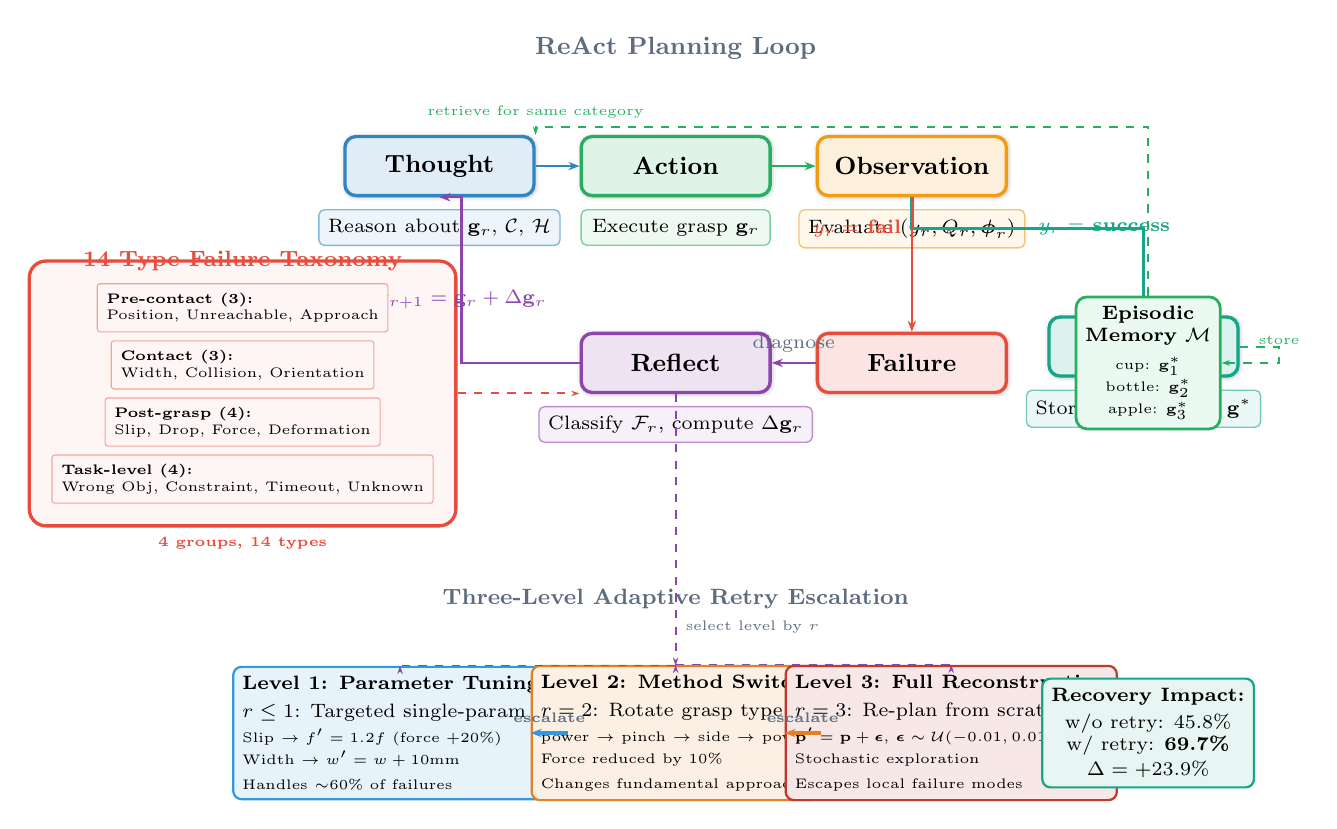
\begin{tikzpicture}[
  >=Stealth,
  node distance=0.4cm,
  reactblock/.style={
    rectangle, rounded corners=4pt,
    draw=#1, fill=#1!15, line width=1.2pt,
    minimum width=2.4cm, minimum height=0.75cm,
    font=\small\bfseries, text=black, align=center,
    blur shadow={shadow blur steps=3, shadow xshift=0.3pt, shadow yshift=-0.3pt}
  },
  smallbox/.style={
    rectangle, rounded corners=2pt,
    draw=#1!60, fill=#1!8, line width=0.5pt,
    font=\scriptsize, text=black, align=center
  },
  levelcard/.style={
    rectangle, rounded corners=3pt,
    draw=#1, fill=#1!12, line width=0.8pt,
    minimum width=2.8cm, minimum height=1.2cm,
    font=\scriptsize, text=black, align=left
  },
  failtype/.style={
    rectangle, rounded corners=1pt,
    draw=failred!50, fill=failred!5, line width=0.4pt,
    font=\tiny, text=black, align=left
  },
  myarrow/.style={
    ->, line width=1pt, color=#1,
    >={Stealth[length=4pt, width=3pt]}
  },
  dashedarrow/.style={
    ->, line width=0.7pt, dashed, color=#1,
    >={Stealth[length=3pt, width=2pt]}
  },
  groupbox/.style 2 args={
    rectangle, rounded corners=6pt,
    draw=#1, fill=#2, line width=1.2pt, inner sep=8pt
  }
]

% ================================================================
% MAIN LOOP: ReAct Cycle (center)
% ================================================================
\node[font=\small\bfseries, text=textgray] at (0, 5.5) {ReAct Planning Loop};

% Thought
\node[reactblock=thoughtblue] (thought) at (-3, 4) {Thought};
\node[smallbox=thoughtblue, below=0.15cm of thought, minimum width=2.4cm] (tdetail)
  {Reason about $\mathbf{g}_r$, $\mathcal{C}$, $\mathcal{H}$};

% Action
\node[reactblock=actiongreen] (action) at (0, 4) {Action};
\node[smallbox=actiongreen, below=0.15cm of action, minimum width=2.4cm] (adetail)
  {Execute grasp $\mathbf{g}_r$};

% Observation
\node[reactblock=obsyellow] (obs) at (3, 4) {Observation};
\node[smallbox=obsyellow, below=0.15cm of obs, minimum width=2.4cm] (odetail)
  {Evaluate $(y_r, Q_r, \boldsymbol{\phi}_r)$};

% Arrows in cycle
\draw[myarrow=thoughtblue] (thought.east) -- (action.west);
\draw[myarrow=actiongreen] (action.east) -- (obs.west);

% Success path
\node[reactblock=successteal, below right=1.5cm and 0.5cm of obs] (success)
  {Success!};
\node[smallbox=successteal, below=0.15cm of success, minimum width=2.2cm] (sdetail)
  {Store in $\mathcal{M}$, return $\mathbf{g}^*$};

\draw[myarrow=successteal, line width=1.2pt] (obs.south) -- ++(0, -0.4) -| (success.north)
  node[near start, right, font=\scriptsize\bfseries, text=successteal] {$y_r = $ success};

% ================================================================
% FAILURE PATH: Reflection
% ================================================================
\node[reactblock=failred] (fail) at (3, 1.5) {Failure};

\draw[myarrow=failred] (obs.south) -- ++(0, -0.4) -| (fail.north)
  node[near start, left, font=\scriptsize\bfseries, text=failred] {$y_r = $ fail};

% Reflection module
\node[reactblock=reflectpurple] (reflect) at (0, 1.5) {Reflect};
\node[smallbox=reflectpurple, below=0.15cm of reflect, minimum width=2.6cm] (rdetail)
  {Classify $\mathcal{F}_r$, compute $\Delta\mathbf{g}_r$};

\draw[myarrow=reflectpurple] (fail.west) -- (reflect.east)
  node[midway, above, font=\scriptsize, text=textgray] {diagnose};

% Back to Thought (retry)
\draw[myarrow=reflectpurple, line width=0.8pt] (reflect.west) -- ++(-1.5, 0) |- (thought.south)
  node[near start, below, font=\scriptsize\itshape, text=reflectpurple] {$\mathbf{g}_{r+1} = \mathbf{g}_r + \Delta\mathbf{g}_r$};

% ================================================================
% FAILURE TAXONOMY (left)
% ================================================================
\node[font=\footnotesize\bfseries, text=failred] at (-5.5, 2.8) {14-Type Failure Taxonomy};

\node[failtype, minimum width=2.8cm] (ft1) at (-5.5, 2.2) 
  {\textbf{Pre-contact (3):}\\Position, Unreachable, Approach};
\node[failtype, minimum width=2.8cm, below=0.1cm of ft1] (ft2)
  {\textbf{Contact (3):}\\Width, Collision, Orientation};
\node[failtype, minimum width=2.8cm, below=0.1cm of ft2] (ft3)
  {\textbf{Post-grasp (4):}\\Slip, Drop, Force, Deformation};
\node[failtype, minimum width=2.8cm, below=0.1cm of ft3] (ft4)
  {\textbf{Task-level (4):}\\Wrong Obj, Constraint, Timeout, Unknown};

\begin{scope}[on background layer]
  \node[groupbox={failred}{failred!5}, fit=(ft1)(ft2)(ft3)(ft4),
    label={[font=\tiny\bfseries, text=failred]below:4 groups, 14 types}] (taxbox) {};
\end{scope}

\draw[dashedarrow=failred] (taxbox.east) -- (reflect.west |- taxbox.east)
  node[midway, above, font=\tiny, text=textgray] {};

% ================================================================
% THREE-LEVEL RETRY (bottom)
% ================================================================
\node[font=\footnotesize\bfseries, text=textgray] at (0, -1.5) {Three-Level Adaptive Retry Escalation};

% Level 1
\node[levelcard=lvl1] (level1) at (-3.5, -3.2)
  {\textbf{Level 1: Parameter Tuning}\\[2pt]
  $r \leq 1$: Targeted single-param fix\\[1pt]
  {\tiny Slip $\to f' = 1.2f$ (force +20\%)}\\
  {\tiny Width $\to w' = w + 10$mm}\\[1pt]
  {\tiny Handles $\sim$60\% of failures}};

% Level 2
\node[levelcard=lvl2] (level2) at (0, -3.2)
  {\textbf{Level 2: Method Switch}\\[2pt]
  $r = 2$: Rotate grasp type\\[1pt]
  {\tiny power $\to$ pinch $\to$ side $\to$ power}\\
  {\tiny Force reduced by 10\%}\\[1pt]
  {\tiny Changes fundamental approach}};

% Level 3
\node[levelcard=lvl3] (level3) at (3.5, -3.2)
  {\textbf{Level 3: Full Reconstruction}\\[2pt]
  $r = 3$: Re-plan from scratch\\[1pt]
  {\tiny $\mathbf{p}' = \mathbf{p} + \boldsymbol{\epsilon}$, $\boldsymbol{\epsilon} \sim \mathcal{U}(-0.01, 0.01)^3$}\\
  {\tiny Stochastic exploration}\\[1pt]
  {\tiny Escapes local failure modes}};

% Escalation arrows
\draw[myarrow=lvl1, line width=1.2pt] (level1.east) -- (level2.west)
  node[midway, above, font=\tiny\bfseries, text=textgray] {escalate};
\draw[myarrow=lvl2, line width=1.2pt] (level2.east) -- (level3.west)
  node[midway, above, font=\tiny\bfseries, text=textgray] {escalate};

% Connection from reflect to levels
\draw[dashedarrow=reflectpurple] (reflect.south) -- ++(0, -1.5) -- (level1.north -| reflect)
  node[near end, right, font=\tiny, text=textgray] {select level by $r$};
\draw[dashedarrow=reflectpurple, line width=0.4pt] (reflect.south |- level1.north) -| (level1.north);
\draw[dashedarrow=reflectpurple, line width=0.4pt] (reflect.south |- level2.north) -- (level2.north);
\draw[dashedarrow=reflectpurple, line width=0.4pt] (reflect.south |- level3.north) -| (level3.north);

% ================================================================
% EPISODIC MEMORY (right side)
% ================================================================
\node[rectangle, rounded corners=4pt, draw=memorybdr, fill=memorybg, 
  line width=1pt, minimum width=1.8cm, minimum height=1.2cm, 
  font=\scriptsize, text=black, align=center] (memory) at (6, 1.5) 
  {\textbf{Episodic}\\
  \textbf{Memory} $\mathcal{M}$\\[2pt]
  {\tiny cup: $\mathbf{g}^*_1$}\\
  {\tiny bottle: $\mathbf{g}^*_2$}\\
  {\tiny apple: $\mathbf{g}^*_3$}};

% Success -> Memory
\draw[dashedarrow=memorybdr] (success.east) -- ++(0.5, 0) |- (memory.east)
  node[near start, above, font=\tiny, text=memorybdr] {store};

% Memory -> Thought  
\draw[dashedarrow=memorybdr] (memory.north) |- ($(thought.east)+(0, 0.5)$) -- (thought.north east)
  node[near start, above, font=\tiny, text=memorybdr] {retrieve for same category};

% ================================================================
% Performance annotation
% ================================================================
\node[rectangle, rounded corners=3pt, draw=successteal, fill=successteal!10,
  line width=0.8pt, font=\scriptsize, align=center] at (6, -3.2) 
  {\textbf{Recovery Impact:}\\[2pt]
  w/o retry: 45.8\%\\
  w/ retry: \textbf{69.7\%}\\[1pt]
  $\Delta = +23.9\%$};

\end{tikzpicture}
\end{document}
